% Student paper — English, typeset text, field diagram as CIE clip. Compiler: XeLaTeX.
% Paper B / 卷B — AB twin of Topic 1 Atomic Structure Exam (Paper A).
\documentclass[10pt,a4paper]{article}

\usepackage[margin=16mm,headheight=13pt,headsep=5pt,footskip=9mm]{geometry}
\usepackage{fontspec}
\usepackage[version=4]{mhchem}
\usepackage{chemfig}
\usepackage{graphicx}
\usepackage{xcolor}
\usepackage{booktabs}
\usepackage{array}
\usepackage{enumitem}
\usepackage{needspace}
\usepackage{fancyhdr}
\usepackage{amsmath,amssymb}
\usepackage{pgffor}
\usepackage{tikz}

\raggedbottom
\setlist[enumerate]{leftmargin=1.5em,itemsep=0.12em,topsep=0.15em,parsep=0pt}
\setlist[itemize]{leftmargin=1.3em,itemsep=0.08em}

\pagestyle{fancy}
\fancyhf{}
\fancyhead[L]{\small \homeworktitle}
\fancyhead[R]{\small \homeworkmarks}
\fancyfoot[C]{\thepage}
\renewcommand{\headrulewidth}{0.3pt}

\newcommand{\homeworktitle}{Chemistry homework}
\newcommand{\homeworkmarks}{}
\newcommand{\sethomework}[2]{%
  \renewcommand{\homeworktitle}{#1}%
  \renewcommand{\homeworkmarks}{#2}%
}

\newcommand{\answerlines}[1]{%
  \par\vspace{0.08em}%
  \foreach \n in {1,...,#1}{\noindent\rule{\linewidth}{0.2pt}\\[0.62em]}%
}

\graphicspath{{images/}}
\DeclareGraphicsExtensions{.png,.jpg,.jpeg,.pdf}

\setlength{\parindent}{0pt}
\setlength{\parskip}{0.10em}
\setlength{\abovedisplayskip}{0.25em}
\setlength{\belowdisplayskip}{0.25em}

\newcommand{\qhead}[2]{%
  \par\vspace{0.28em}%
  \Needspace{4.2em}%
  \noindent{\small\textbf{#1}}\hfill{\small[#2]}\par\vspace{0.08em}%
}

\begin{document}
\sethomework{AS Chemistry --- Topic 1 Atomic Structure (Exam · Paper B)}{33 marks}

\begin{center}
{\large\bfseries AS Chemistry --- Topic 1 Atomic Structure (Exam · Paper B)}\\[0.12em]
{\small CIE 9701 AS Chemistry · Paper B · 33 marks · about 40--45 minutes}
\end{center}

{\small Topic 1: particles and isotopes, mass spectrometry, electronic configuration / orbitals, and ionisation energy.
Answer in English. Section A is Paper 1 style (1 mark each). Section B is written; show working and give the usual CIE reasons (nuclear charge, radius, shielding, spin-pair repulsion) where asked. A Periodic Table may be used.}

\vspace{0.15em}
{\small
\begin{tabular}{@{}llr@{}}
\toprule
\textbf{Section} & \textbf{Content} & \textbf{Marks} \\
\midrule
A & Multiple choice & 13 \\
B1 & Iron isotopes, $A_\mathrm{r}$, configuration and particles & 10 \\
B2 & Tellurium: sub-shell and successive ionisation energy & 6 \\
B3 & Mass spectrum of hydrocarbon R: $n(\mathrm{C})$ and a fragment & 4 \\
\midrule
 & \textbf{Total} & \textbf{33} \\
\bottomrule
\end{tabular}}

\vspace{0.30em}
{\large\bfseries Section A --- Multiple-choice questions (13 marks)}\par

\qhead{A1.}{1}
{\small Which statement about \ce{^{131}_{53}I} is correct?}
\begin{enumerate}[label=\textbf{\Alph*}, leftmargin=1.7em, itemsep=0.08em]
\item A negative ion of \ce{^{131}_{53}I} contains 53 neutrons and 52 electrons.
\item A negative ion of \ce{^{131}_{53}I} contains 53 neutrons and 54 electrons.
\item A negative ion of \ce{^{131}_{53}I} contains 78 neutrons and 52 electrons.
\item A negative ion of \ce{^{131}_{53}I} contains 78 neutrons and 54 electrons.
\end{enumerate}

\qhead{A2.}{1}
{\small Technetium (Tc) is a second row transition element that does not occur naturally on Earth. One of its isotopes has 56 neutrons.}

{\small What is the nucleon number of this isotope?}\par
\vspace{0.06em}
{\small
\begin{tabular}{@{}p{0.22\linewidth}p{0.22\linewidth}p{0.22\linewidth}p{0.22\linewidth}@{}}
\textbf{A} 43 & \textbf{B} 56 & \textbf{C} 99 & \textbf{D} 112
\end{tabular}}
\par

\Needspace{14em}
\qhead{A3.}{1}
{\small In which row do the particles increase in size?}

\vspace{0.10em}
\centering
{\small
\begin{tabular}{cccc}
\toprule
 & smallest & $\longrightarrow$ & largest \\
\midrule
\textbf{A} & N & O & F \\
\textbf{B} & \ce{N^{3-}} & \ce{O^{2-}} & \ce{F-} \\
\textbf{C} & \ce{Na+} & \ce{Mg^{2+}} & \ce{Al^{3+}} \\
\textbf{D} & \ce{Na+} & Ne & \ce{F-} \\
\bottomrule
\end{tabular}}
\par\raggedright

\Needspace{18em}
\qhead{A4.}{1}
{\small A helium ion contains two protons, two neutrons and one electron.}

{\small This helium ion and a proton are passed separately through a uniform electric field.}

{\small The particles are travelling at the same velocity.}

{\small Which arrow describes the path of each particle?}

\vspace{0.08em}
\begin{center}

\includegraphics[width=0.58\linewidth,keepaspectratio]{fig-a4-field.png}
\end{center}

\vspace{0.08em}
\centering
{\small
\begin{tabular}{ccc}
\toprule
 & helium ion & proton \\
\midrule
\textbf{A} & 1 & 2 \\
\textbf{B} & 2 & 1 \\
\textbf{C} & 4 & 5 \\
\textbf{D} & 5 & 4 \\
\bottomrule
\end{tabular}}
\par\raggedright

\qhead{A5.}{1}
{\small A sample of magnesium contains the isotopes \ce{^{24}Mg}, \ce{^{25}Mg} and \ce{^{26}Mg} only.}

{\small The percentage abundance of \ce{^{25}Mg} and \ce{^{26}Mg} is the same.}

{\small The relative atomic mass of magnesium in the sample is 24.3.}

{\small What is the percentage abundance of \ce{^{24}Mg}?}
\vspace{0.06em}
{\small
\begin{tabular}{@{}p{0.22\linewidth}p{0.22\linewidth}p{0.22\linewidth}p{0.22\linewidth}@{}}
\textbf{A} 10\% & \textbf{B} 20\% & \textbf{C} 60\% & \textbf{D} 80\%
\end{tabular}}
\par

\Needspace{12em}
\qhead{A6.}{1}
{\small What is the electronic configuration for the particle \ce{^{27}_{13}Al+}?}
\vspace{0.06em}
{\small
\begin{tabular}{@{}p{0.46\linewidth}p{0.46\linewidth}@{}}
\textbf{A} \ce{1s^2 2s^2 2p^6 3s^1 3p^1} & \textbf{B} \ce{1s^2 2s^2 2p^6 3s^2} \\[0.12em]
\textbf{C} \ce{1s^2 2s^2 2p^6 3s^2 3p^2} & \textbf{D} \ce{1s^2 2s^2 2p^6 3s^2 3p^6 3d^7 4s^1}
\end{tabular}}
\par

\Needspace{12em}
\qhead{A7.}{1}
{\small Which statement about a 3p orbital is correct?}
\begin{enumerate}[label=\textbf{\Alph*}, leftmargin=1.7em, itemsep=0.08em]
\item It can hold a maximum of six electrons.
\item It has the highest energy of the orbitals with principal quantum number 3.
\item It is at a higher energy level than a 3s orbital but has the same shape.
\item It is occupied by one electron in an isolated phosphorus atom.
\end{enumerate}

\Needspace{10em}
\qhead{A8.}{1}
{\small In which pair of species do both species have only one unpaired p electron?}
\vspace{0.06em}
{\small
\begin{tabular}{@{}p{0.46\linewidth}p{0.46\linewidth}@{}}
\textbf{A} \ce{Ar+} and \ce{C-} & \textbf{B} B and \ce{Ti+} \\[0.12em]
\textbf{C} F and Ga & \textbf{D} \ce{Se-} and \ce{Si-}
\end{tabular}}
\par

\Needspace{12em}
\qhead{A9.}{1}
{\small Why is the first ionisation energy of oxygen less than that of nitrogen?}
\begin{enumerate}[label=\textbf{\Alph*}, leftmargin=1.7em, itemsep=0.08em]
\item The nitrogen atom has its outer electron in a different subshell.
\item The nuclear charge on the oxygen atom is greater than that on the nitrogen atom.
\item The oxygen atom has a pair of electrons in one p orbital that repel one another.
\item There is more shielding in an oxygen atom.
\end{enumerate}

\Needspace{14em}
\qhead{A10.}{1}
{\small The second ionisation energy of oxygen is greater than the second ionisation energy of fluorine.}

{\small Which factor explains this difference?}
\begin{enumerate}[label=\textbf{\Alph*}, leftmargin=1.7em, itemsep=0.08em]
\item The atomic radius of an oxygen atom is smaller than that of fluorine.
\item The covalent bond in a fluorine molecule is weaker than the bond in an oxygen molecule.
\item A spin-paired electron is removed from fluorine but \textbf{not} from oxygen.
\item Fluorine has more electrons in total than oxygen. This causes a greater shielding of the nuclear attraction in fluorine.
\end{enumerate}

\Needspace{12em}
\qhead{A11.}{1}
{\small The first seven ionisation energies of an element between lithium and neon in the Periodic Table are shown.}

\vspace{0.08em}
\centering
{\small 1310 \quad 3390 \quad 5320 \quad 7450 \quad 11000 \quad 13300 \quad 71000 \quad kJ\,mol$^{-1}$}
\par\raggedright

\vspace{0.10em}
{\small What is the outer electronic configuration of the element?}
\vspace{0.06em}
{\small
\begin{tabular}{@{}p{0.46\linewidth}p{0.46\linewidth}@{}}
\textbf{A} \ce{2s^2} & \textbf{B} \ce{2s^2 2p^1} \\[0.12em]
\textbf{C} \ce{2s^2 2p^4} & \textbf{D} \ce{2s^2 2p^6}
\end{tabular}}
\par

\qhead{A12.}{1}
{\small Which of these elements has the highest fifth ionisation energy?}
\vspace{0.06em}
{\small
\begin{tabular}{@{}p{0.22\linewidth}p{0.22\linewidth}p{0.22\linewidth}p{0.22\linewidth}@{}}
\textbf{A} C & \textbf{B} N & \textbf{C} P & \textbf{D} Si
\end{tabular}}
\par

\Needspace{14em}
\qhead{A13.}{1}
{\small The first ionisation energy of potassium, K, is 418\,kJ\,mol$^{-1}$. The first ionisation energy of strontium, Sr, is 548\,kJ\,mol$^{-1}$.}

{\small Which statement helps to explain why Sr has a greater first ionisation energy than K?}
\begin{enumerate}[label=\textbf{\Alph*}, leftmargin=1.7em, itemsep=0.08em]
\item The charge on a Sr nucleus is greater than the charge on a K nucleus.
\item The outer electron in a Sr atom experiences greater shielding than the outer electron in a K atom.
\item The outer electron in a Sr atom experiences spin-pair repulsion.
\item The outer electron in a Sr atom is further from the nucleus than the outer electron in a K atom.
\end{enumerate}

\clearpage
% Tighter Section B only: keep stems at \small (~9–10pt) and fit B1–B3 on two pages.
\renewcommand{\answerlines}[1]{%
  \par\vspace{0.02em}%
  \foreach \n in {1,...,#1}{\noindent\rule{\linewidth}{0.2pt}\\[0.40em]}%
}
\renewcommand{\qhead}[2]{%
  \par\vspace{0.10em}%
  \Needspace{3.0em}%
  \noindent{\small\textbf{#1}}\hfill{\small[#2]}\par\vspace{0.02em}%
}

{\large\bfseries Section B --- Structured questions (20 marks)}\par\vspace{0.06em}
{\normalsize\bfseries B1 · Iron isotopes, relative atomic mass, configuration and particles (10 marks)}\par

{\small A sample of iron contains three different isotopes and has a relative atomic mass, $A_\mathrm{r}$, of 55.8.}

\qhead{B1(a)(i)}{2}
{\small Define relative atomic mass.}
\answerlines{3}

\Needspace{10em}
\qhead{B1(a)(ii)}{2}
{\small Table 2.1 shows the abundances of two of the isotopes present in the sample of iron.}

\vspace{0.04em}
\centering
{\small
\begin{tabular}{lcc}
\toprule
isotope & relative isotopic mass & abundance / \% \\
\midrule
\ce{^{54}Fe} & 53.9 & 6.0 \\
\ce{^{56}Fe} & 55.9 & 91.9 \\
\bottomrule
\end{tabular}}
\par\vspace{0.02em}
{\small Table 2.1}\par
\raggedright

{\small Use Table 2.1 to calculate the relative isotopic mass of the third isotope of iron in the sample.}

{\small Show your working.}
\answerlines{3}
{\small relative isotopic mass = \underline{\hspace{3.2cm}}}

\qhead{B1(b)}{1}
{\small Deduce the number of pairs of electrons in the 3d sub-shell in an iron(II) ion.}
\vspace{0.08em}
{\small number of pairs of electrons \underline{\hspace{3.2cm}}}

\Needspace{6em}
\qhead{B1(c)}{1}
\noindent
\begin{minipage}[c]{0.58\linewidth}
{\small Sketch the shape of the lowest energy orbital in the shell with principal quantum number $n = 2$.}
\end{minipage}%
\hfill
\fbox{\begin{minipage}[c][2.15cm][c]{3.2cm}\centering\mbox{}\end{minipage}}

\Needspace{8em}
\qhead{B1(d)}{2}
{\small Complete Table 2.2 to show information about particles in one ion of \ce{^{56}Fe^{3+}}.}

\vspace{0.04em}
\centering
{\small
\begin{tabular}{|p{3.6cm}|p{7.0cm}|}
\hline
particle & number of particles present in one ion of \ce{^{56}Fe^{3+}} \\
\hline
electrons & \vspace{0.55em} \\
\hline
\vspace{0.55em} & 30 \\
\hline
\end{tabular}}
\par\vspace{0.02em}
{\small Table 2.2}\par
\raggedright

\Needspace{8em}
\qhead{B1(e)}{2}
{\small The atomic radius of iron is $1.26 \times 10^{-10}$\,m.}

{\small Suggest the change to the radius, if any, after an iron atom reacts to produce an \ce{Fe^{3+}} ion.}

{\small Explain your answer.}
\answerlines{4}

\vspace{0.16em}
{\normalsize\bfseries B2 · Tellurium: sub-shell and successive ionisation energy (6 marks)}\par

{\small Tellurium is an element in Group 16. The most common isotope of tellurium is \ce{^{130}Te}. Its electronic configuration is $[\mathrm{Kr}]\,4\mathrm{d}^{10}\,5\mathrm{s}^{2}\,5\mathrm{p}^{4}$.}

\qhead{B2(a)}{1}
{\small Identify the sub-shell in an atom of Te that contains electrons with the lowest energy.}
\vspace{0.08em}
{\small sub-shell \underline{\hspace{3.2cm}}}

\Needspace{5em}
\qhead{B2(b)}{1}
{\small Construct an equation to represent the first ionisation energy of Te.}
\answerlines{2}

\Needspace{8em}
\qhead{B2(c)(i)}{2}
{\small The radius of Te ions decreases after each successive ionisation.}

{\small State \textbf{two} factors that are responsible for the increase in the first six ionisation energies of Te.}
\answerlines{4}

\Needspace{10em}
\qhead{B2(c)(ii)}{2}
{\small Sketch a graph in Fig.\ 1.1 to show the trend in the first \textbf{seven} ionisation energies of Te.}

\vspace{0.04em}
\begin{center}
\begin{tikzpicture}[x=0.78cm,y=0.44cm]
  \draw[->] (0,0) -- (0,6.4);
  \draw[->] (0,0) -- (8.05,0);
  \node[rotate=90,anchor=south,font=\small] at (-0.90,3.2) {ionisation energy / kJ\,mol$^{-1}$};
  \node[font=\small,anchor=north] at (4.0,-0.55) {successive ionisation};
  \node[left,font=\small] at (0,0) {0};
  \foreach \x in {0,1,...,7} {
    \draw (\x,0.08) -- (\x,-0.08);
  }
  \foreach \x in {1,2,...,7} {
    \node[below,font=\small] at (\x,-0.08) {\x};
  }
\end{tikzpicture}\\[0.06em]
{\small Fig.\ 1.1}
\end{center}

\vspace{0.10em}
{\normalsize\bfseries B3 · Mass spectrum of hydrocarbon R (4 marks)}\par

{\small P, Q and R are three different hydrocarbon molecules.}

{\small The mass spectrum of hydrocarbon R is recorded. Information about the two peaks with $m/e$ greater than 135 is shown in Fig.\ 6.1.}

\vspace{0.04em}
\begin{center}
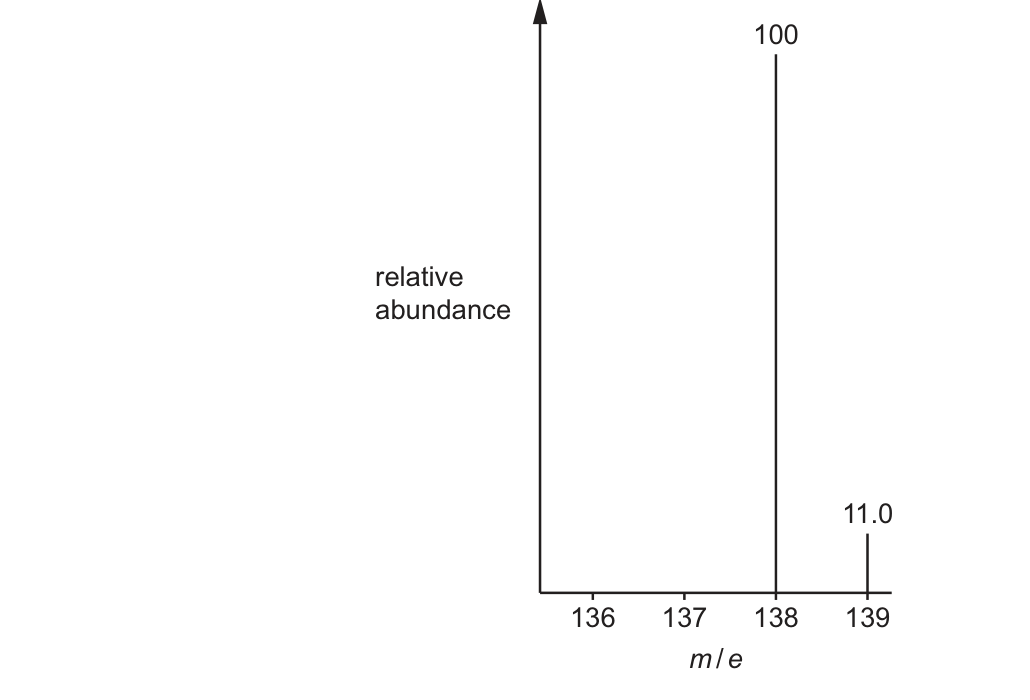
\includegraphics[height=3.55cm,keepaspectratio]{fig-b3-spectrum.png}\\[0.04em]
{\small Fig.\ 6.1}
\end{center}

\Needspace{6em}
\qhead{B3(a)}{2}
{\small Use Fig.\ 6.1 to deduce the number of carbon atoms in a molecule of R.}

{\small Show your working.}
\answerlines{2}
{\small number of carbon atoms = \underline{\hspace{3.2cm}}}

\Needspace{4em}
\qhead{B3(b)}{1}
{\small Use Fig.\ 6.1 and your answer to (a) to deduce the molecular formula of R.}
\answerlines{2}

\Needspace{4em}
\qhead{B3(c)}{1}
{\small Suggest the molecular formula of the fragment of R with $m/e = 57$.}
\answerlines{2}

\end{document}
